\chapter{Approach}\label{ch:approachPerspective}
This chapter will provide an overview of how an approach to having a robot explore Mars and what future perceptive can be in exploring Mars, human colonization of Mars?


\section{Approach}
Talking about how to approach having a robotic explorer on Mars, it is needed to take in the many different variables when comparing Mars to Earth. Variables such as gravity, surface, radiation, weather, atmosphere, how much sunlight reaches Mars surface, and how the robot can navigate and map the area most efficiently. These parameters will help us determine the solution with chances of a working robot arriving on Mars and not breaking down due to unforeseen circumstances.\\
It is needed to know about the gravity as a factor, since it is very important that the robot can drive around in unknown environment, that is on Mars. It is therefore also important to know how the robots weight will impact its driving on Mars, since the gravity on Mars will make the robots weight seem different than on Earth.\\ 
The wheels for the robot will be chosen due to the surface on Mars, which is why it is important to consider how the soil on Mars will have a impact on the wheels. It is wanted that all wheels will remain on the surface to have traction and maneuverability. The surface will also have an impact on the way that suspension is designed and which kind of motor to use to make sure that the robot has a chance of moving.\\
The knowledge of the atmosphere on Mars, is of utmost importance, since the chemical composition will have influence on what material is going to be used for the robot. If the atmosphere is acidic, then the robot has to wear a non-corroding body, and the cables and wires must not dissolve and produce a short-circuit.\\ 
The atmosphere will have an impact on how much sunlight reaches the surface. This helps determine what kind of power source the robot should depend on. If enough sunlight shines through, the robot could run on solar panels, if not another option like Radioisotope Thermo-electric Generator could be used.\\
It is also important to know the radiation level on Mars. The robots may have to be radioactive hardened to sustain its mission, if there is a high level of alpha rays, beta rays and gamma rays on Mars, the robot may need to be shielded. Earth are protected by the core of Earth magnetic properties.
The robot will have different sensors attached to it, so it can examine the terrain and move around on Mars safely. What solution will be best suitable for the robot to have, will be determined beforehand, when it is known what Mars is like, and what is needed for the robot to move around, avoid obstacles and do the mapping and navigation of this\cite{WhatAreCosmicRays?}\cite{mmtg}.

%\section{Perspective}
%Is it possible for humans to live on Mars?
%When thinking the Earth might not last forever and the human survival instinct wants to find another solution as of living on another planet. There is still a lot of research needed to be done, before questions like these can be answered.
%Right now robots are patrolling the environment on Mars and exploring new territory, this will be described in more detail in chapter \ref{ch:existingSolutions}. 
%A robot, with the right components can patrol around on Mars with no risk to itself. It is not alive like humans and therefore does not need air to breathe or food to eat. As it is now, NASA have not yet discovered what ingredients there is in the water on Mars, and if it even is drinkable\cite{Curiosity2016}.


%Mars is only half the size of Earth, and there's only a part of the planet there's inhabitable, since the gravity is different all over the planet.\cite{howbigismars}\cite{gravity}
%As seen on figure \ref{fig:image003.jpg}, Earth and Mars are compared to each other as to the differences between the days in a year, gravity, sunlight and atmosphere.

%\begin{figure}[h]
%    \centering
%    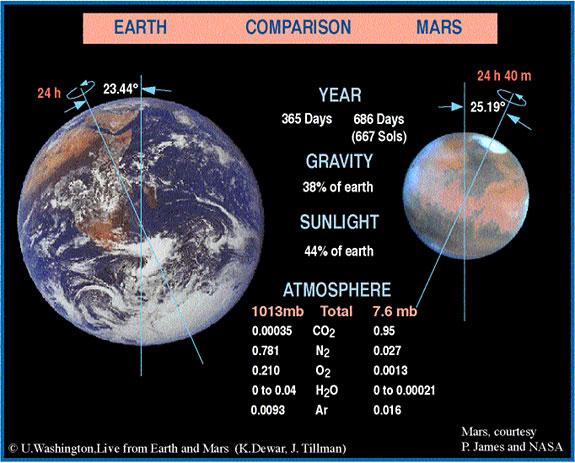
\includegraphics[width=.8\linewidth]{figures/image003.jpg}
%    \caption{Earth and Mars comparison \cite{gravity}}
%    \label{fig:image003.jpg} 
%\end{figure}


